\chapter{The physics behind sailboats}
%In \cite{philpott1993yacht} and \cite{larsonprinciples} agree that the essential or basic principles about the mechanics of sailing have been know since 1950's, and in 1979 Marchaj  published a book, \cite{marchaj1979aero} to compile and review the available knowledge about sailing and add information which is still being used for yacht design, like coefficients and other calculations. Because  sailboats move through 2  different fluids it is important to know how the elements are named and which words are related with specific maneuvers.  These simple concepts, will help you to understand how the equilibrium is generated in the static and steady  state, what elements interacts on it and how the balance is conserved when the sailboat moves from one point to another. 
Sailing boats are propelled mainly by wind, however they displace through the water; in other words, sailboats move through 2 different fluids: water and wind. The mechanics of sailing have been know since 1950's.  Marchaj in 1979 review them and add information which is still being used for yacht design \cite{marchajaereo1979}.\par 

This chapter is focus on the motion of the sailboats, what are physics behind, which forces interact in equilibrium and during motion. How the athlete takes part of this model and what other consideration are required to set-up the equations of motion. Since sailboats are govern by similar equations some adjustments are required to differentiate between yachts and lasers this adjustments are explained at the end of the chapter. The equations of motion facilitate the identification of variables that can be use as a parameter to model the trajectory as well as to identify its limitations. These considerations are required to optimize the trajectory and obtain the minimal time path. \par
\section{Interaction between the sailboat, water and air} \label{sec:interaction_boat_environ}
The origin of the forces and momentum depends on the interaction of the elements of the sailboat with the 2 mediums, water and air. Some of this forces are clear, like the forces acting above the water surface which are produced by the wind and the interaction of it with the sails. These forces have to be balanced by the forces beneath the same surface; in this case, the water interacts with the hull, rudder and keel. Therefore by adjusting the sail and the rudder, the only movable elements, the sailboat can hold a steady course.\par

Philpott explains how different elements, parts of the sailboat, interact with the surroundings and how they are used to control and attain the equilibrium during motion. Figure \ref{sailboat_terms} shows the most common elements and where are they located. Some of those elements can be manipulated by the seamanship, which means that the variables concerned can be controlled and therefore they are know as control variables \cite{philpott1993yacht}. \par
%In addition, 
%The main elements of the sailboat, including wind, currents and waves were grouped in 3 categories that affect the equilibrium in a different way \cite{philpott1993yacht}.
 %\begin{enumerate} \label{factorphil}
% \setlength \itemsep{0em}
% \item Environmental factors; such as wind and current intensity and direction,
% \item Design factor, dimensions that characterize the type of boat. 
 %\item Control variables, variables affecting by the seamanship
 %\end{enumerate}
 \begin{figure}%[ht]
\centering
  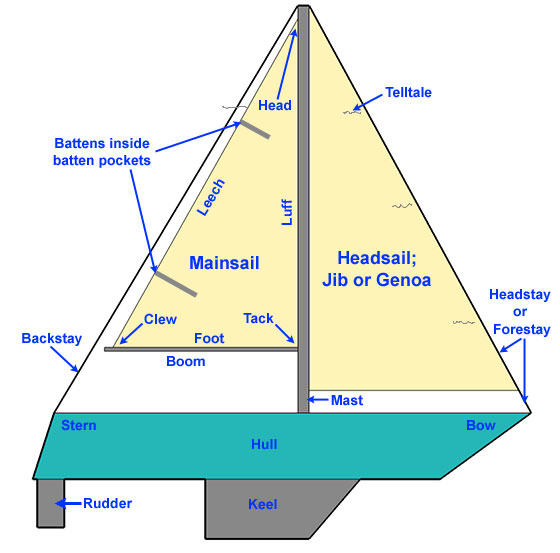
\includegraphics[width=0.4\linewidth]{sailboat_terms.jpg}
 \caption{Common sailboat terms \cite{sailboat_terms}. }
\label{sailboat_terms}
\end{figure}
In order to steer a boat the seamanship has to control the angle of the rudder, this interacts directly with the current, the direction obtained is called \textit{heading} and these two, rudder and current, generate forces that influence the boat to \textit{yaw}. \par
Due to the wind direction, mainly, the boat slip sideways and this effect is know as \textit{leeway}. The difference in course comparing with the heading is expressed as \textit{leeway angle ($\lambda$)}. %, which can be see in the figure \ref{forces_m} \textit{C}.
The sails adjustment is known as trim; when the trim reduce the area of the sail then the seaman is \textit{reefing}, most of the time this term refers when the size of the sails is changing.  Reefing under sail allows the seamanship to control the wind intensity. \par
The wind over the sails, generates a force and an angle called \textit{heel angle}; which can be see in the figure \ref{forces_m} \textit{B}, this decrease the driving force. Under those circumstances, a moment is generated and to neutralize it, the seamanship generates a \textit{righting moment} (\textit{ $M_{R}$}) by standing on the windward side of the boat to produce it\cite{philpott1993yacht}. %A graphical representation of the interaction of these forces is  found in \ref{forces_m}.
As a result of these forces, the velocity could be optimal or not. \cite{larsonprinciples} relates the factors and forces proposed in\cite{philpott1993yacht} in terms of forces and resistances, indicating how the dynamics of each of the mediums, water and air, interact to keep the balance (and be capable to maximize the boat's speed). Therefore, the forces and resistances are related as showed below: \par 
\begin{itemize}  \label{milgramforces}
 \setlength \itemsep{0em}
\item Aerodynamic driving forces = Hydrodynamic resistance;
\item Aerodynamic side force = Hydrodynamic side force;
\item Aerodynamic heeling moment=Hydrodynamic (static) righting moment.
\end{itemize}
An important assumption made by  \cite{philpott1993yacht} and \cite{larsonprinciples} to keep the analysis of the boat in 2 dimensions is that vertical forces are in balance always, same as the pitching moment; Figure \ref{forces_m} \textbf{c} shows the only forces that acts when this assumption is made; additionally 2 angles are shown, one of then refers to the wind.\par

\section{Planes of motion}
Sailing boats are considered rigid bodies that can move in a three dimensional space; figure \ref{DOF} shows the 6 fundamental types of motion or degrees of freedom (DOF)  with the names and axis where they are referred: three translations and three rotations. \par 
It also shows the water surface which is represented by the plane \textit{XY} and the orientation of the sailboat shows the positive direction of the three axes which follow the right-hand orthogonal system. Thus, \textit{X} axis is positive in the direction of the motion, \textit{Y} is positive to port or left side of the sailboat and \textit{Z} is positive upwards. In the case of the \textit{Y} axis the negative direction or right side of the sailboat is know as starboard.  Besides, for future references, the speed of the boat is along the \textit{X} axis. These six DOF correspond to three forces and three moments which are going to explain in the next section. \par 
\begin{figure} %[ht]
\centering
  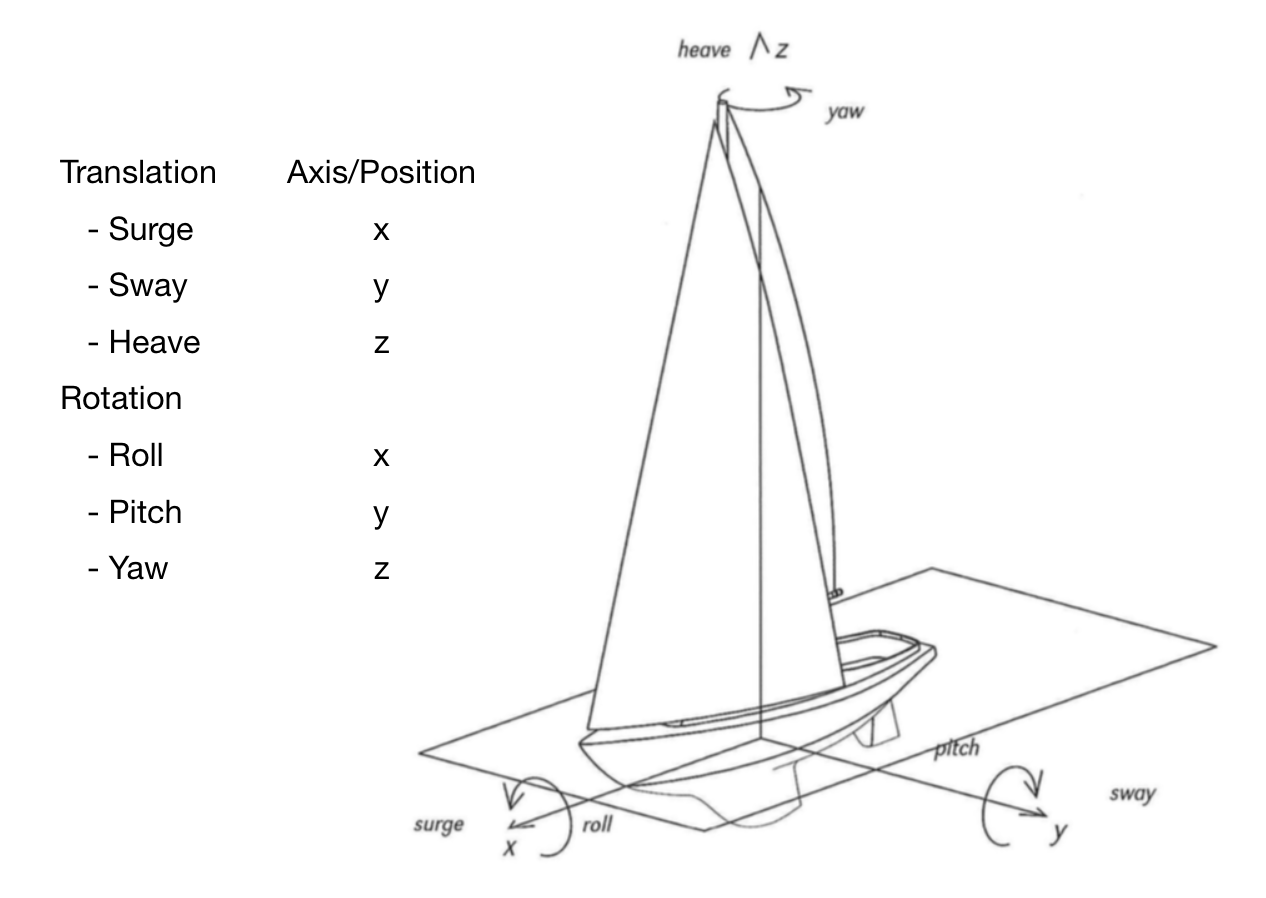
\includegraphics[width=0.7\linewidth]{dof_foss_modif.png}
 \caption{Degrees of freedom of a boat, clockwise reference system xyz \cite{fossati2009aero}. }
\label{DOF}
\end{figure}

Because the sail boat interact between two fluids not only they generate forces but also resistances in both mediums. It is important to know how the elements are named and which words are related with specific axis.  These simple concepts are useful to understand how the equilibrium is generated in the static condition, what elements interacts on it and how it is conserved when the sailboat moves from one point to another. \par 

\section{Hydrodynamic and Aerodynamic Forces and Momentum} \label{section:forces_moment}
The static and dynamic balance of any type of boat is based on Newton's second law. However, when the boat moves, a dynamic situation, it is the winds' velocity that leads this equilibrium. Because the sail boat interact between two fluids they not only  generate forces but also resistances.
The next equations basically show that the total aerodynamic force ($F_{A}$) is equal and opposite to the total hydrodynamic force ($F_{H_{TOT}}$). \par

\subsection{Wind and the Velocity Triangle} \label{subsec:wind_vel_trian}
In sailing, the wind is characterized by its speed and direction and it is defined as \textit{true wind ($_{tw}$)} and \textit{true wind angle ($\beta_{tw}$)}.  Because it also interacts with the water surface, in some cases its intensity depends on the height where it was measured, to know its value at different height it is estimated by the equation \ref{eq:wind_h}. According \cite{claughton1998sailing} the exponent $\kappa$ has a value between 1/7 and 1/14; and the reference height for measurements is 10m above the water surface. \par 
\begin{equation} \label{eq:wind_h}
    V_{tw}(Z)=V_{tw}(Z_{ref}) \cdot \bigg( \frac{Z}{Z_{ref}} \bigg)^\kappa
\end{equation}

The steady motion of the sailboat not only depends on the balance of forces but also on the relation between velocities, boat and wind, mainly. This interaction is represented by the velocity triangle shown in figure \ref{vel_triangle}. The triangle introduce the apparent wind velocity ($V_{aw}$) and angle ($\beta_{aw}$).\par 
\begin{figure}[ht]
\centering
  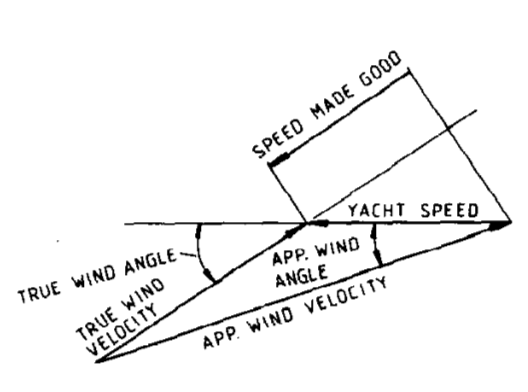
\includegraphics[width=0.65\linewidth]{Larsson_triang_vel.png}
 \caption{Velocity triangle  \cite{larsonprinciples}. }
\label{vel_triangle}
\end{figure}
The $V_{aw}$ and $\beta_{aw}$ result from the vector summation of the true wind ($V_{tw}$) and sailboat ($V_{boat}$) velocities; to estimate them it uses the heel angle ($\Theta$), equations \ref{eq:app_angle} and \ref{eq:app_angle} show how to calculate them. These equations include the heel angle because $V_{aw}$ are used to calculate some sail force coefficients which are specified at center of effort (\textit{CE}),its location is about 40\% at the mast height. The $\beta_{aw}$ incorporated the leeway angle ($\lambda$), which value is usually less than 6\degree \cite{philpott1993yacht},\cite{claughton1998sailing}. \par
\begin{equation} \label{eq:app_angle}
    \beta_{aw}=tan^{-1} \bigg( \frac{ V_{tw} sin \beta_{tw} cos \Theta }{ V_{tw} cos \beta_{tw} + V_{boat}} \bigg)
\end{equation}
\newline
\begin{equation} \label{eq:ap_vel}
    V_{aw}=  \sqrt{ (V_{tw} sin \beta_{tw} cos \Theta)^2 + (V_{tw} cos \beta_{tw} + V_{boat})^2}
\end{equation}
\subsection {Equilibrium Equations} \label{section_equil_equat}
In static condition, the equilibrium is reach when the summation of all the forces and momentum equals zero. In figure \ref{forces_m} these forces are located according the planes where they act, the names of them and the fluid that drives them. In addition to the forces and momentum, there are 4 angles to consider. Another observation is how the position and weight of the athlete is incorporated in the equilibrium equations. \par 

The equations of force(\textit{F}) by plane in equilibrium are:
\begin{equation}\label{eq:force_x}
    \text{(Surge, x  \space axis)  \space} F_{R}=R \\
\end{equation}
\begin{equation}\label{eq:force_y}
    \text{(Sway, y\space axis) \space } \space F_{H,lat}=F_{S,lat}\\
\end{equation}
\begin{equation}\label{eq:force_z}
    \text{(Heave, z\space axis)  } \space F_{V}=F_{VW}
\end{equation}
And the those for the momentum (\textit{M}) in equilibrium are:
\begin{equation}\label{eq:m_x}
    \text{(Roll, x  \space axis) \space } M_{R}=M_{H} \\
\end{equation}
\begin{equation}\label{eq:m_y}
    \text{(Pitch, y \space axis)  } \space M_{PA}=F_{PW}\\
\end{equation}
\begin{equation}\label{eq:m_z}
    \text{(Yaw, z \space axis)  } \space M_{YW}=M_{YL}
\end{equation}

 \begin{figure}[ht]
\centering
  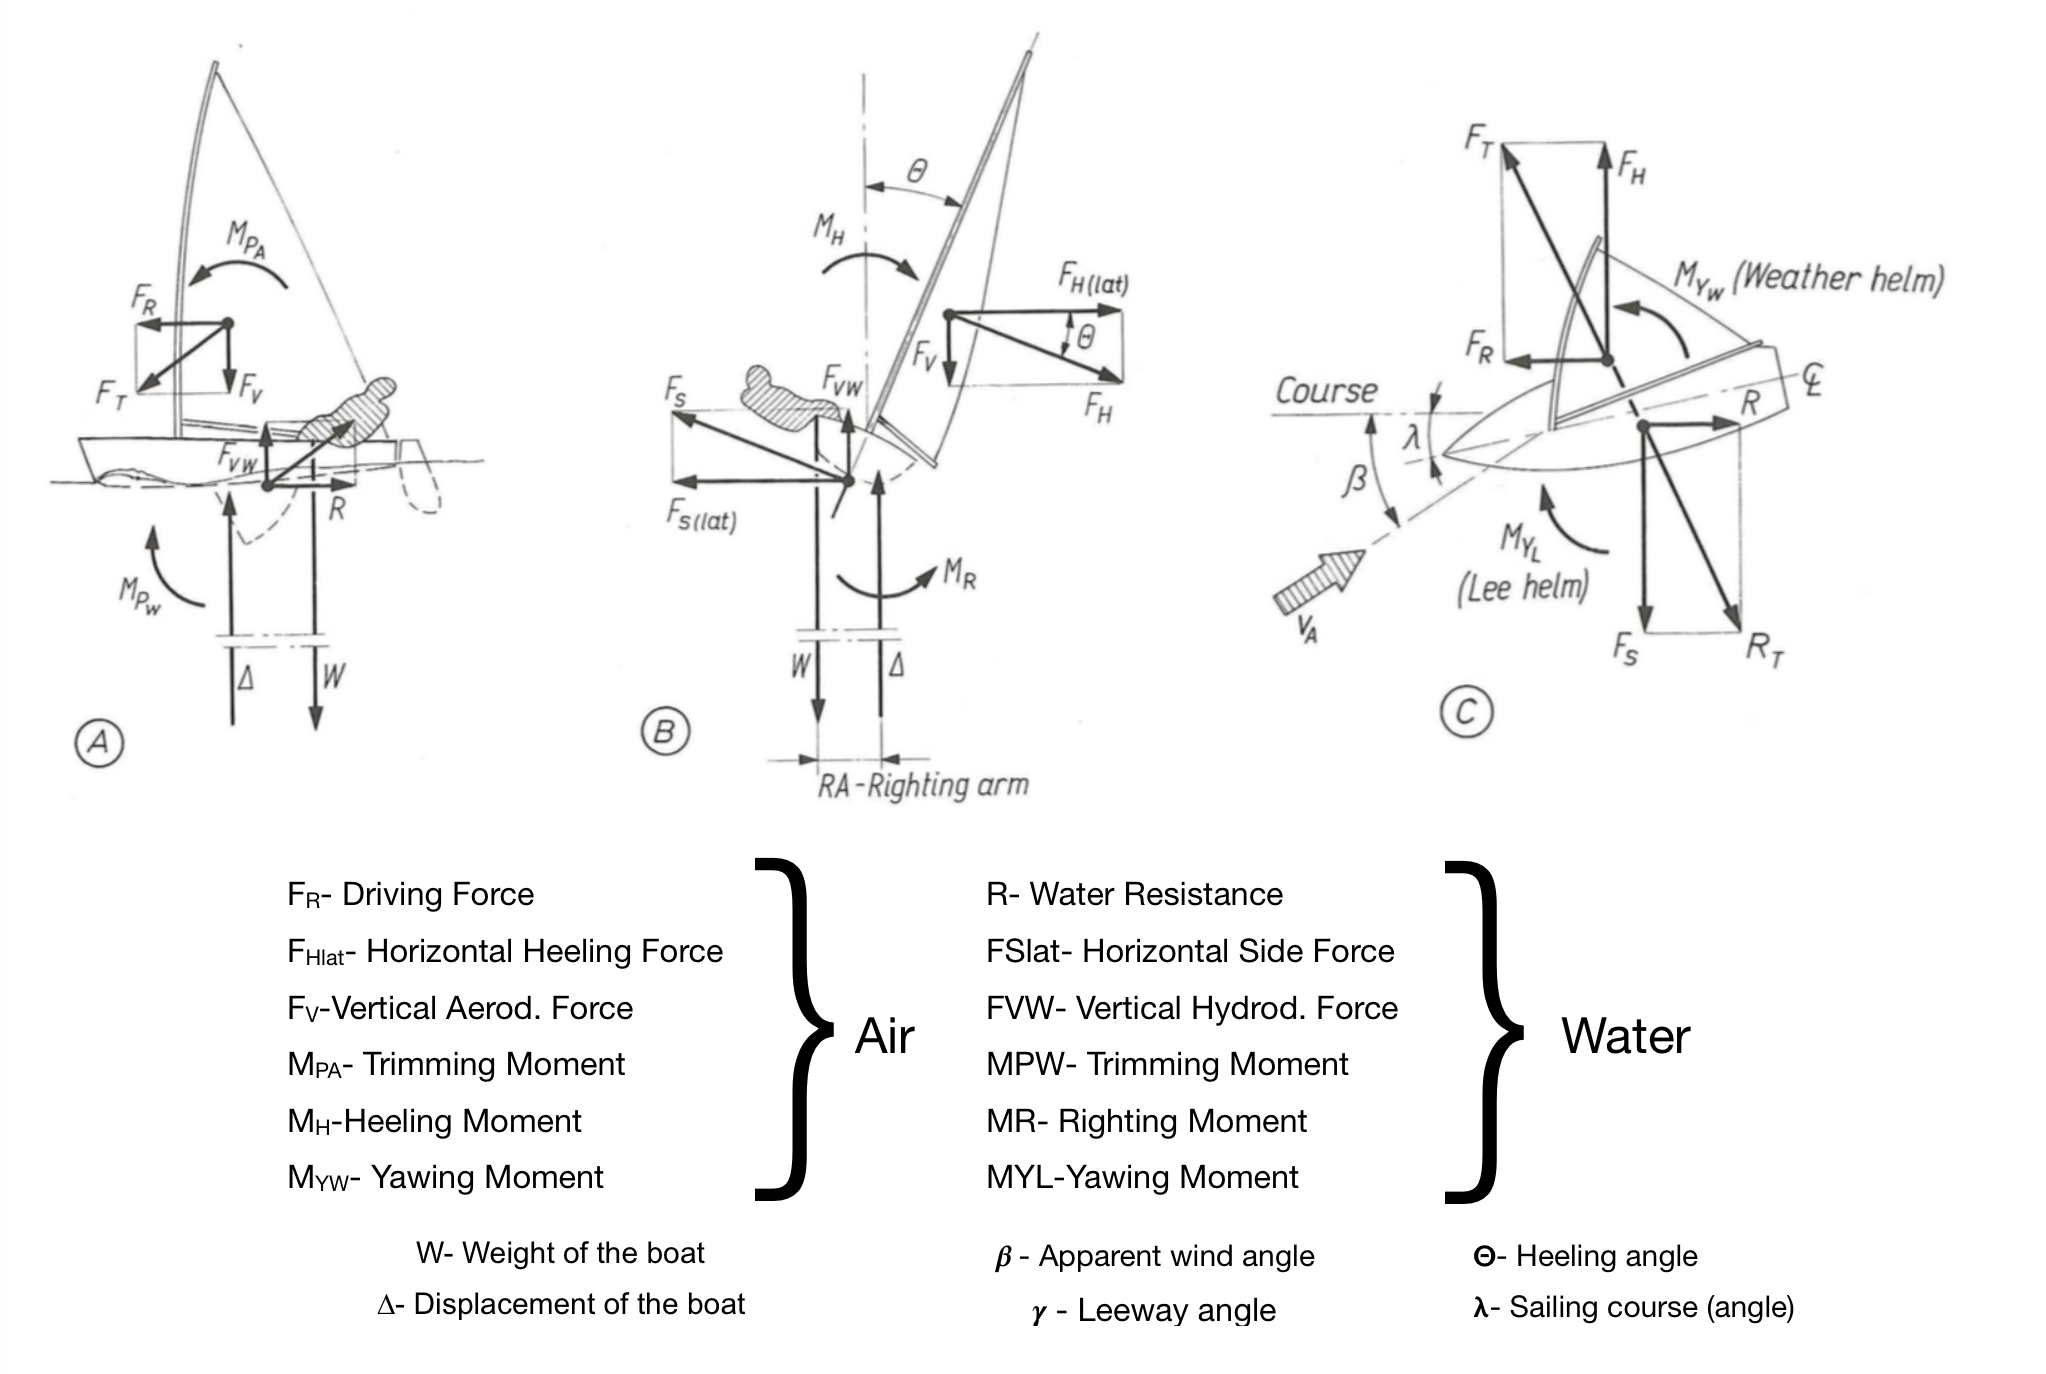
\includegraphics[width=.97\linewidth]{marchaj_forces.png}
 \caption{Equilibrium of forces and moments in steady-state sailing condition \cite{marchajaereo1979} }
\label{forces_m}
\end{figure}

\subsection{Aerodynamic Forces and Resistances}
The force that drives motion of the sailboat is the driving force($F_{R}$); figure \ref{forces_m} \textit{B} shows the force that causes the drift (heel) of the sailboat is the heeling force ($F_{H}$). The motion of the sailboat happens when $F_{R}$ beat the hull resistance (\textit{R}); while in the \textit{ZY} plane the balance of the forces happens when $F_{H}$ equals the hydrodynamic side force ($F_{S}$), which is produced by the effect of the water over the hull. Then:\par 

( Because $F_{A}$ result from $F_{R}$, parallel to the \textit{apparent wind} direction and $F_{H}$ perpendicular to $F_{R}$. Under balance the variables related to them are:)
\begin{multline}
\\
F_{A}=F_{R}(\parallel V_{aw}) + F_{H}(\bot F_{R} )\\
F_{R}=F_{R}(V_{aw},\beta_{a}, \Theta) \\
F_{H}=F_{R}(V_{aw},\beta_{a}, \Theta) \\
F_{S_{lat}}=F_{S}(V_{boat},\lambda, \Theta) \\
R=R(V_{boat},\lambda, \Theta)\\  
\end{multline}
\\
%th they depend on the $V_{aw}$ and $\beta_{a}$; while $F_{S}$ and \textit{R} depend on $V_{boat}$ and $\lambda$. 
Due to the dependency on velocities, $F_{R}$ and $F_{H}$ generate drag (\textit{D}) and lift (\textit{L}) forces acting normal to the centre plane of the hull and mast and they are integrated in to the forces, according to \cite{philpott1993yacht} and \cite{claughton1998sailing} as: \par 
\begin{equation} \label{eq:Fr_LD}
    F_{R}=L sin \beta_{a} - D cos \beta_{a}
\end{equation}
\begin{equation} \label{eq:Fh_LD}
    F_{H}=(L cos \beta_{a} + D sin \beta_{a}) cos\Theta
\end{equation}
\\ \textit{D} and \textit{L} depends not only depends on  the sail area (\textit{$A_{s}$)}, $V_{aw}$, and fluid density ($\rho_{a}$), in this case air, but also on coefficients which depends on the trim and flatness of the sail \cite{philpott1993yacht}, \cite{carrico17symp}, \cite{day2017performance}; these last, are under the control of the seamanship. \textit{D} and \textit{L}  are expressed in those terms as follow: \par
\begin{equation} \label{eq:Lift}
  L=qA_{s}C_{t}  
\end{equation}
\begin{equation} \label{eq:Draf}
    D=qA_{s}C_{d}  
\end{equation}
\begin{equation} \label{eq:dynamic_press}
    q=\frac{1}{2}\rho_{a} V_{aw}^2
\end{equation}
\begin{equation} \label{eq:Cd}
    C_{d}=C_{d}(\beta_{a},trim, flatness)
\end{equation}
\begin{equation} \label{eq:Ct}
    C_{t}=C_{t}(\beta_{a},trim, flatness)
\end{equation}
where:
\begin{itemize} \label{ae_symbols}
    \item $\rho_{a}$ air density approx. 1.225 $kg/m^3$.
    \item $A_{s}$ is the area of the sail.
\end{itemize}

$C_{d}$ and $C_{t}$ values are obtained from tables or graphics and their range is over (0,1), later on this is going to be explain in detail. \par 
$F_{R}$ is the total force applied on the sail which can be decompose in 2 more forces; a driven force $F_{ms}$ and a side force $F_{ss}$ expressed in the terms mentioned before as:\par
\begin{equation}\label{eq:drive_sail_force}
    F_{ms}= (L cos \beta_{a}+ D sin \beta_{a})cos \Theta sin \lambda + (L sin \beta_{a}-D cos\beta_{a})cos \lambda
\end{equation}
\begin{equation}\label{eq:side_sail_force}
    F_{ss}=(L cos \beta_{a}+ D sin \beta_{a})cos \Theta cos \lambda - (L sin \beta_{a}-D cos\beta_{a})sin \lambda
\end{equation}
%%%NEW SUBSECTION %%%
\subsection {Hydrodynamic Forces and Resistances}
$F_{H_{TOT}}$ is equivalent to $F_{A}$ with the difference that they result from the interaction with the water. In this case, \textit{R}, a drag force (resistance) oppose to the motion of the sailboat; and the horizontal side force $F_{S_{lat}}$, is a lift force acting over the hull and keel. Most of the information related with the modelling of the hull and keel is based on experimental data% which is used to calibrate the theoretical model.
Then the drag generated by the hull is the result of: the  upright,heeled and induced resistances \cite{philpott1993yacht}.\par
\begin{equation}
    F_{H_{TOT}}=R(\parallel( -V_{aw})) + F_{S_{lat}}(\bot R )\\
\end{equation}
%The hull drag when $\lambda$ is zero produces the upright resistance.
The upright resistance is produced by the hull drag and when $\lambda$ is zero. It is constituted by the friction generated by the water viscosity and wave drag, a dissipation of energy in form of waves due to the shape of the hull.  The  formula to calculate these two frictional forces, equation \ref{eq:water_fric} and \ref{eq:wave_fric} is similar to the one from classical hydrodynamics, the difference are the coefficients. $C_{f}$ depends on $V_{boat}$ and its waterline length while $C_{w}$ depends on the hull shape and Froude number (\textit{Fr}), which considers the $V_{boat}$ and length of the sailboat; however it is often determine by tests evaluations.
\begin{equation}\label{eq:water_fric}
 F_{f}=\frac{1}{2}\rho_{w} C_{f} A_{w} V_{boat}^2
\end{equation}
\begin{equation}\label{eq:wave_fric}
 F_{w}=\frac{1}{2}\rho_{w} C_{w} A_{w} V_{boat}^2
\end{equation}
where:
\begin{itemize} \label{R_symbols}
    \item $\rho_{w}$ water density approx. 1000 $kg/m^3$.
    \item $A_{w}$ is the wetted surface are of the sailboat
\end{itemize}
The induced and heeled resistances are combined and related with the heel and $\lambda$, its formula depends also depends on $V_{boat}$. Due to its complex derivation and different versions the expression is going to be set as; $F_{i}(\lambda,\Theta,V_{boat})$, for the purpose of this work. Then \textit{R} due to hydrolic resistances is calculated as: \par 
\begin{equation} \label{eq:R_total}
    R=F_{f}+F_{w}+F_{i}
\end{equation}

In the case of $F_{S_{lat}}$, it depends also on 3 resistances generated by the hull, the lifting surface of the rudder and keel; these 2 last are the more significant and they are also perpendicular to the velocity. This total side force (\textit{S}), on the water plane, depends on the plan area of the keel and rudder and in 2 coefficients,respectively.  Thus, it is estimated as: \par 
\begin{equation}
    S=\frac{1}{2} \rho_{w} V_{boat}^2(C_{rudder}A_{rudder}+C_{keel}A_{keel})cos \Theta
\end{equation}.
The shape, of the rudder and keel, in conjunction with the angle of attack has implication on each coefficients respectively. %$C_{rudder}$ and $C_{keel}$, each depends on the the shape and angle of attack of each. 
The angle of the rudder ($\beta_{r}$) is the angle it makes with the center line of the sailboat. Each angle of attack (\textit{$\beta_{i_{a}}$})is determine as: \par 
\begin{equation}
    \beta_{r_{a}}=tan ^{-1} (cos \Theta cos \lambda + \beta_{r})
\end{equation}
\begin{equation}
    \beta_{k_{a}}=tan ^{-1} (cos \Theta cos \lambda
\end{equation}

$F_{S_{lat}}$ in equilibrium can be estimated based by using $F_{H}$ which generates a reaction force below the water surface, then: %
which us know as horizontal side force $F_{Slat}$ and it is determined as follow: \par
\begin{equation}
    F_{Slat}= F_{H}cos \Theta
\end{equation}
% review to insert an image to express the relation on the moments by plane  from philpott 
%% new section
\subsection{Momentum at the sailboat model}
Because $F_{A}$ is apply at \textit{CE}, above the waterline and located over the sails area; and $F_{H_Tot}$ at the center of lateral resistance (\textit{CLR}),defined below the waterline. The moments generated over the sailboat depends on these 4 variables. For example, the \textit{righting moment ($M_{R}$)}, figure \ref{forces_m} \textit{B} is counterbalanced as next: 
\begin{equation}\label{eq:right_mom}
    M_{R}=F_{H}(CE-CLR)_{z}=W \cdot RA
\end{equation}
where:\par
\begin{itemize}
    \item $(CE-CLR)_{z}$ is the heeling arm or the vertical distance between \textit{CE} and \textit{CLR} when $F_{H}$ is perpendicular to it.
    \item W = weight of the boat.
    \item RA = Righting arm or the horizontal distance between the \textit{W} and the \textit{Z} axis.
\end{itemize}

This expression does not take into account the weight of the crew. The moment generated by the crew weight is given by the weight of the crew (\textit{$W_{c}$})) and its relative position to the centerline of the boat, which is expressed by a variable know as \textit{$y_{c}$}. This variable has a range value of [-1,1], and if the crew is in the centerline then its value is zero. Another factor to considers is $\Theta$. So the moment generated by the crew according Philpott \cite{philpott1993yacht} is: \par 
\begin{equation}\label{eq:Moment_crew}
    M_{c} = y_{c} W_{c} Y_{max} cos \Theta
\end{equation} 
\begin{equation} \label{eq:Mcrew_dist}
    Y_{max} = \frac{1}{2} beam(width)_{sailboat}
\end{equation}

and the \textit{total righting moment ($M_{R_{TOT}}$)} is:
\begin{equation} \label{eq:Mr_tot}
    M_{R_{TOT}}=M_{R}(V_{boat}, \Theta, \lambda) + M_{c}
\end{equation}

The \textit{yaw moment} $(M_{Y})$ causes the rotation on the \textit{Z} axis and depends most of time, on the rudder angle (\textit{$\beta_{r}$}) since it can shifts the \textit{CLR}, another form to change this distance is by trimming which change the area of the sail therefore the \textit{CE} shifts its location. If the sailing motion is steady then this moment is zero; otherwise, it can be calculated by the hydrodynamic resistance from the hull and the from the keel and rudder side forces; which are compensated by the sail forces \cite{philpott1993yacht}, \cite{claughton1998sailing}. These 3 forces generated the $(M_{Y})$, as shown next: \par
\begin{equation}\label{eq:Hull_R}
    R_{hull}=R+F_{H}=F_{f}+F_{w}+F_{H}
\end{equation}
\begin{equation}\label{eq:hull_moment}
   M_{hull}=R_{hull}(CLR_{y} cos \lambda sin \Theta - x_{y} sin \lambda cos \Theta) 
\end{equation}
\begin{equation}\label{eq:keel-rudder_moment}
   M_{k-r}=\frac{1}{2}\rho_{w} V_{boat}^2(C_{rudder}A_{rudder}x_{r}+C_{keel}A_{keel}x_{k})cos \Theta cos \lambda
\end{equation}
\begin{equation}\label{eq:sail_moment}
    M_{sail}=x_{s}F_{ss}+z_{0}r sin \Theta F_{ms}) cos \lambda
\end{equation}

The \ref{eq:hull_moment} uses $x_{y}$ which refers to the distance of the \textit{CLR} from the \textit{Z} axis (\textit{yaw axis}) while in \ref{eq:keel-rudder_moment} $x_{r}$ and $x_{k}$ are the lever arms of the rudder and keel, respectively, finally in \ref{eq:sail_moment} $x_{s}$ is the distance from the yaw axis to the \textit{CE} and $z_{0}r$ is the lever arm of it, where $z_{0}$ is the height of the \textit{CE}  and \textit{r} is the reefed/trim proportion of the sail. As mentioned in section \ref{subsec:wind_vel_trian} $\lambda$ is small which allows that cos and sin functions can be simplify by linear approximations. \par 
The \textit{trimming moment} ($M_{P}$) arise from gravity (\textit{g}) and buoyancy forces, the displacement of the boat (\textit{$\Delta$}) is related with $V_{boat}$ ; for example, at high velocities the lift forces are added to the buoyancy forces at the front sections. 
%Becuase $F_{A}$ and of the drag (\textit{D}) and lift (\textit{L}) forces generated by the wind on the sail, more specific the \textit{apparent wind}. (\textit{D}) is at the same direction as the \textit{apparent wind} while (\textit{L}) is perpendicular to (\textit{D}). \par 
In case of rough water, however the pitching motion reduces the speed and it is compensated by the aerodynamic and hydrodynamic forces\cite{claughton1998sailing}.\par % by both mediums,% Another consideration refers to the wind, the force it generates over the sails is applied at  the center of effort on them which is assumed to be located at 40\% of the mast height \cite{philpott1993yacht}. \par 

%while in a dynamic situation, as when the boats moves, it is the velocity that leads this equilibrium%.
The equilibrium of forces and moments of the sailboat results from the interaction between the forces generated by the air, or by  water or by both into different parts of the sailboat. These interactions in some cases are sophisticated. One of the reasons are the values that depends on coefficients related with the shape of particular element of the sailboat and the condition of the wind besides the fact that the density value of each medium is different. The steady motion is reached when all this forces are in equilibrium considering the wind and its direction. Due to the complexity of the relation above the solution or equilibrium condition is not unique. Because of these, it is possible to sail at different directions and to reach a place even when it is on on the windward side of the sailboat. % which is explained in the next section.%winda elements it is possible to know the velocity of the sailboat at different directions respect to the wind
%%% NEW SECTION%%%%%
\section{Velocity Prediction Polar} \label{sec:VPP}
In 1979 scientist developed the velocity prediction  program (\textit{VPP}) with the objective to predict the sailboat speed and direction for any wind condition, magnitude and direction \cite{larsonprinciples}. The results can be interpreted easily using a polar diagram or by reading its results in the form of tables.  The kinetics of the sailboat explains how the motive forces from sails equals the hull resistance and how side forces from keel and rudder equal the sail side forces; in other words, how the aerodynamic forces and momentum are counterbalance by the hydrodynamics of it. These relations, and results are obtaining from the static equilibrium equations mentioned in section \ref{section_equil_equat}.\par 
The VPP contains the solutions of the equations to  accomplish this balance and it requires not only to solve the hydrodynamic and aerodynamic equations but also to know the properties of the sailboat related with its stability, such as $\lambda$ \cite{larsonprinciples}, \cite{milgram1998fluid}. The information required to get a VPP comes from different sources and all the variables involved can be classified in 4 categories or groups, according to \cite{philpott1993yacht} these groups are:
\begin{itemize}
    \item design (\textit{$_{d}$}): describe the size and shape of the sailboat and its elements.
    \item environment (\textit{$_{e}$}): describe the wind and current in which the sailboat will perform.
    \item control (\textit{$_{x_{c}}$}): these are setting variables that can be adjusted within some limits or constraints by the seamanship, such as $\beta_{r}$, $y_{c}$, \textit{f} and \textit{r}.
    \item behaviour (\textit{$_{y_{b}}$}): these variables describes the motion or condition of the motion at a given time or due to a given environmental condition. Examples of this type or variables are: $\lambda$, $\beta_{tw}$, $\Theta$ and the $V_{boat}$
\end{itemize}
The rest of the variables can be group as \textit{auxiliary} variables (\textit{$_{aux}$}). These variables describe transitional stages or intermediate calculations, such as $V_{aw}$, \textit{D}, \textit{L}, $M_{c}$, $M_{sail}$ among others. The arrangement of these groups results in at least 22 simultaneous nonlinear equations which can be solve by specifying a performance criterion and optimizing the \textit{$_{y_{b}}$} variables.
%From the equations of previous sections 18 variables were identiy as \textit{aux}.  
 
Because VPP plots are symmetric only half of it is usually represented as shown in the figure \ref {typ_vpp}. The polar diagram indicates the wind direction or \textit{true wind angle} at 0\degree , $V_{boat}$ is defined by the radius size of the concentric half circles, the straight lines indicates the direction of the boat from the wind direction. Last, 
%the angle direction between the wind and the boat. The result
the wind speed are the lines that form a half heart shape; the intersection of these lines with direction lines, indicates the maximum velocity that a sailboat can attain. \par 
\begin{figure} %[ht]
  \centering
  \subfloat[VPP plot for true wind angles from 0 \degree to 180\degree and true wind speeds from 4 to 10 m/s (7.77-19.44 kn) \cite{larsonprinciples}.]{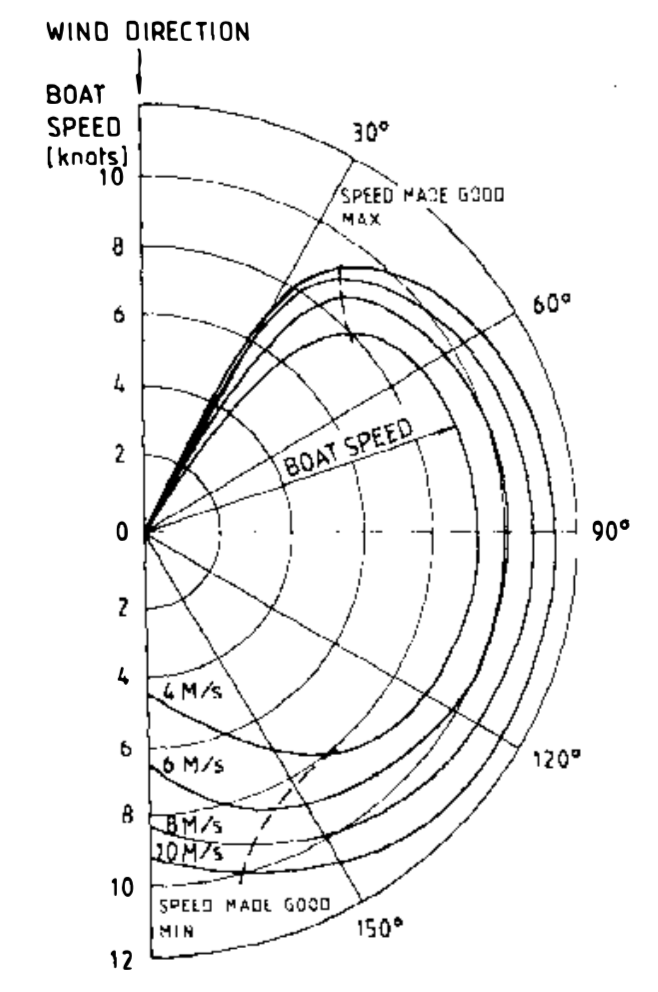
\includegraphics[width=0.38\textwidth]{vppLarsson1990.png}\label{typ_vpp}}
  \hfill
  \subfloat[Polar Curve of the Propulsion System \cite{yang2011control}(Full VPP representation).]{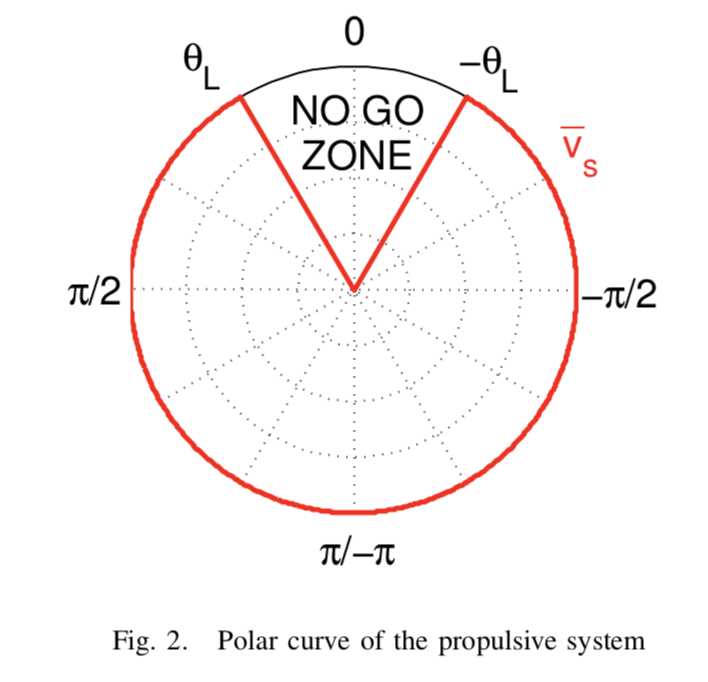
\includegraphics[width=0.45\textwidth]{no-go_zone_yang.png}\label{no_go_zone}}
  \caption{VPP diagram}
\label{vpp_diag} 
\end{figure}

By using the VPP not only the direction of the maximum sailboat speed can be identify but also it shows the direction where the speed is the slowest. The angle range of this speed or speeds corresponds to the concave curve of the true wind, the area is defined as the \textit{no go-zone} and it represents the set of directions that should be avoid to stay away from the irons \cite{yang2011control},\cite{denny2009float}, which means that under these directions the sailboat  motion is minimal, its propulsion is no enough or minimal to outweigh the resistance derived from the hull and sail.\par 

The performance criterion most used is to maximize $V_{boat}$ except when the sailing is towards the wind, upwind condition or sailing to windward. In this case the performance criterion change from velocity to the distance that can be travel during certain time.  This criteria is known as the velocity made good \textit{(VMG)} and it indicates where the sailboat is on the space from a reference and how is its motion \cite{larsonprinciples}, \cite{marchajaereo1979} \cite{philpott1993yacht}. \textit{VMG} is determine by the equation \ref{eq:VMG}. This relation can also be found in the velocity triangle, figure \ref{vel_triangle}, a more detailed geometrical is the figure \ref{fig:vmg_marchal_book}, where it is possible to identify how the $\beta_{tw}$ and $\lambda$ interact to gets the $\beta_{aw}$ therefore how distance from the origin or reference point can be optimized and how different angles perform with the same given time. \par

\begin{equation}\label{eq:VMG}
\begin{aligned}
VMG &=  \mid V_{boat} cos \beta_{tw} \mid 
\end{aligned}
\end {equation}

\begin{figure}
    \centering
    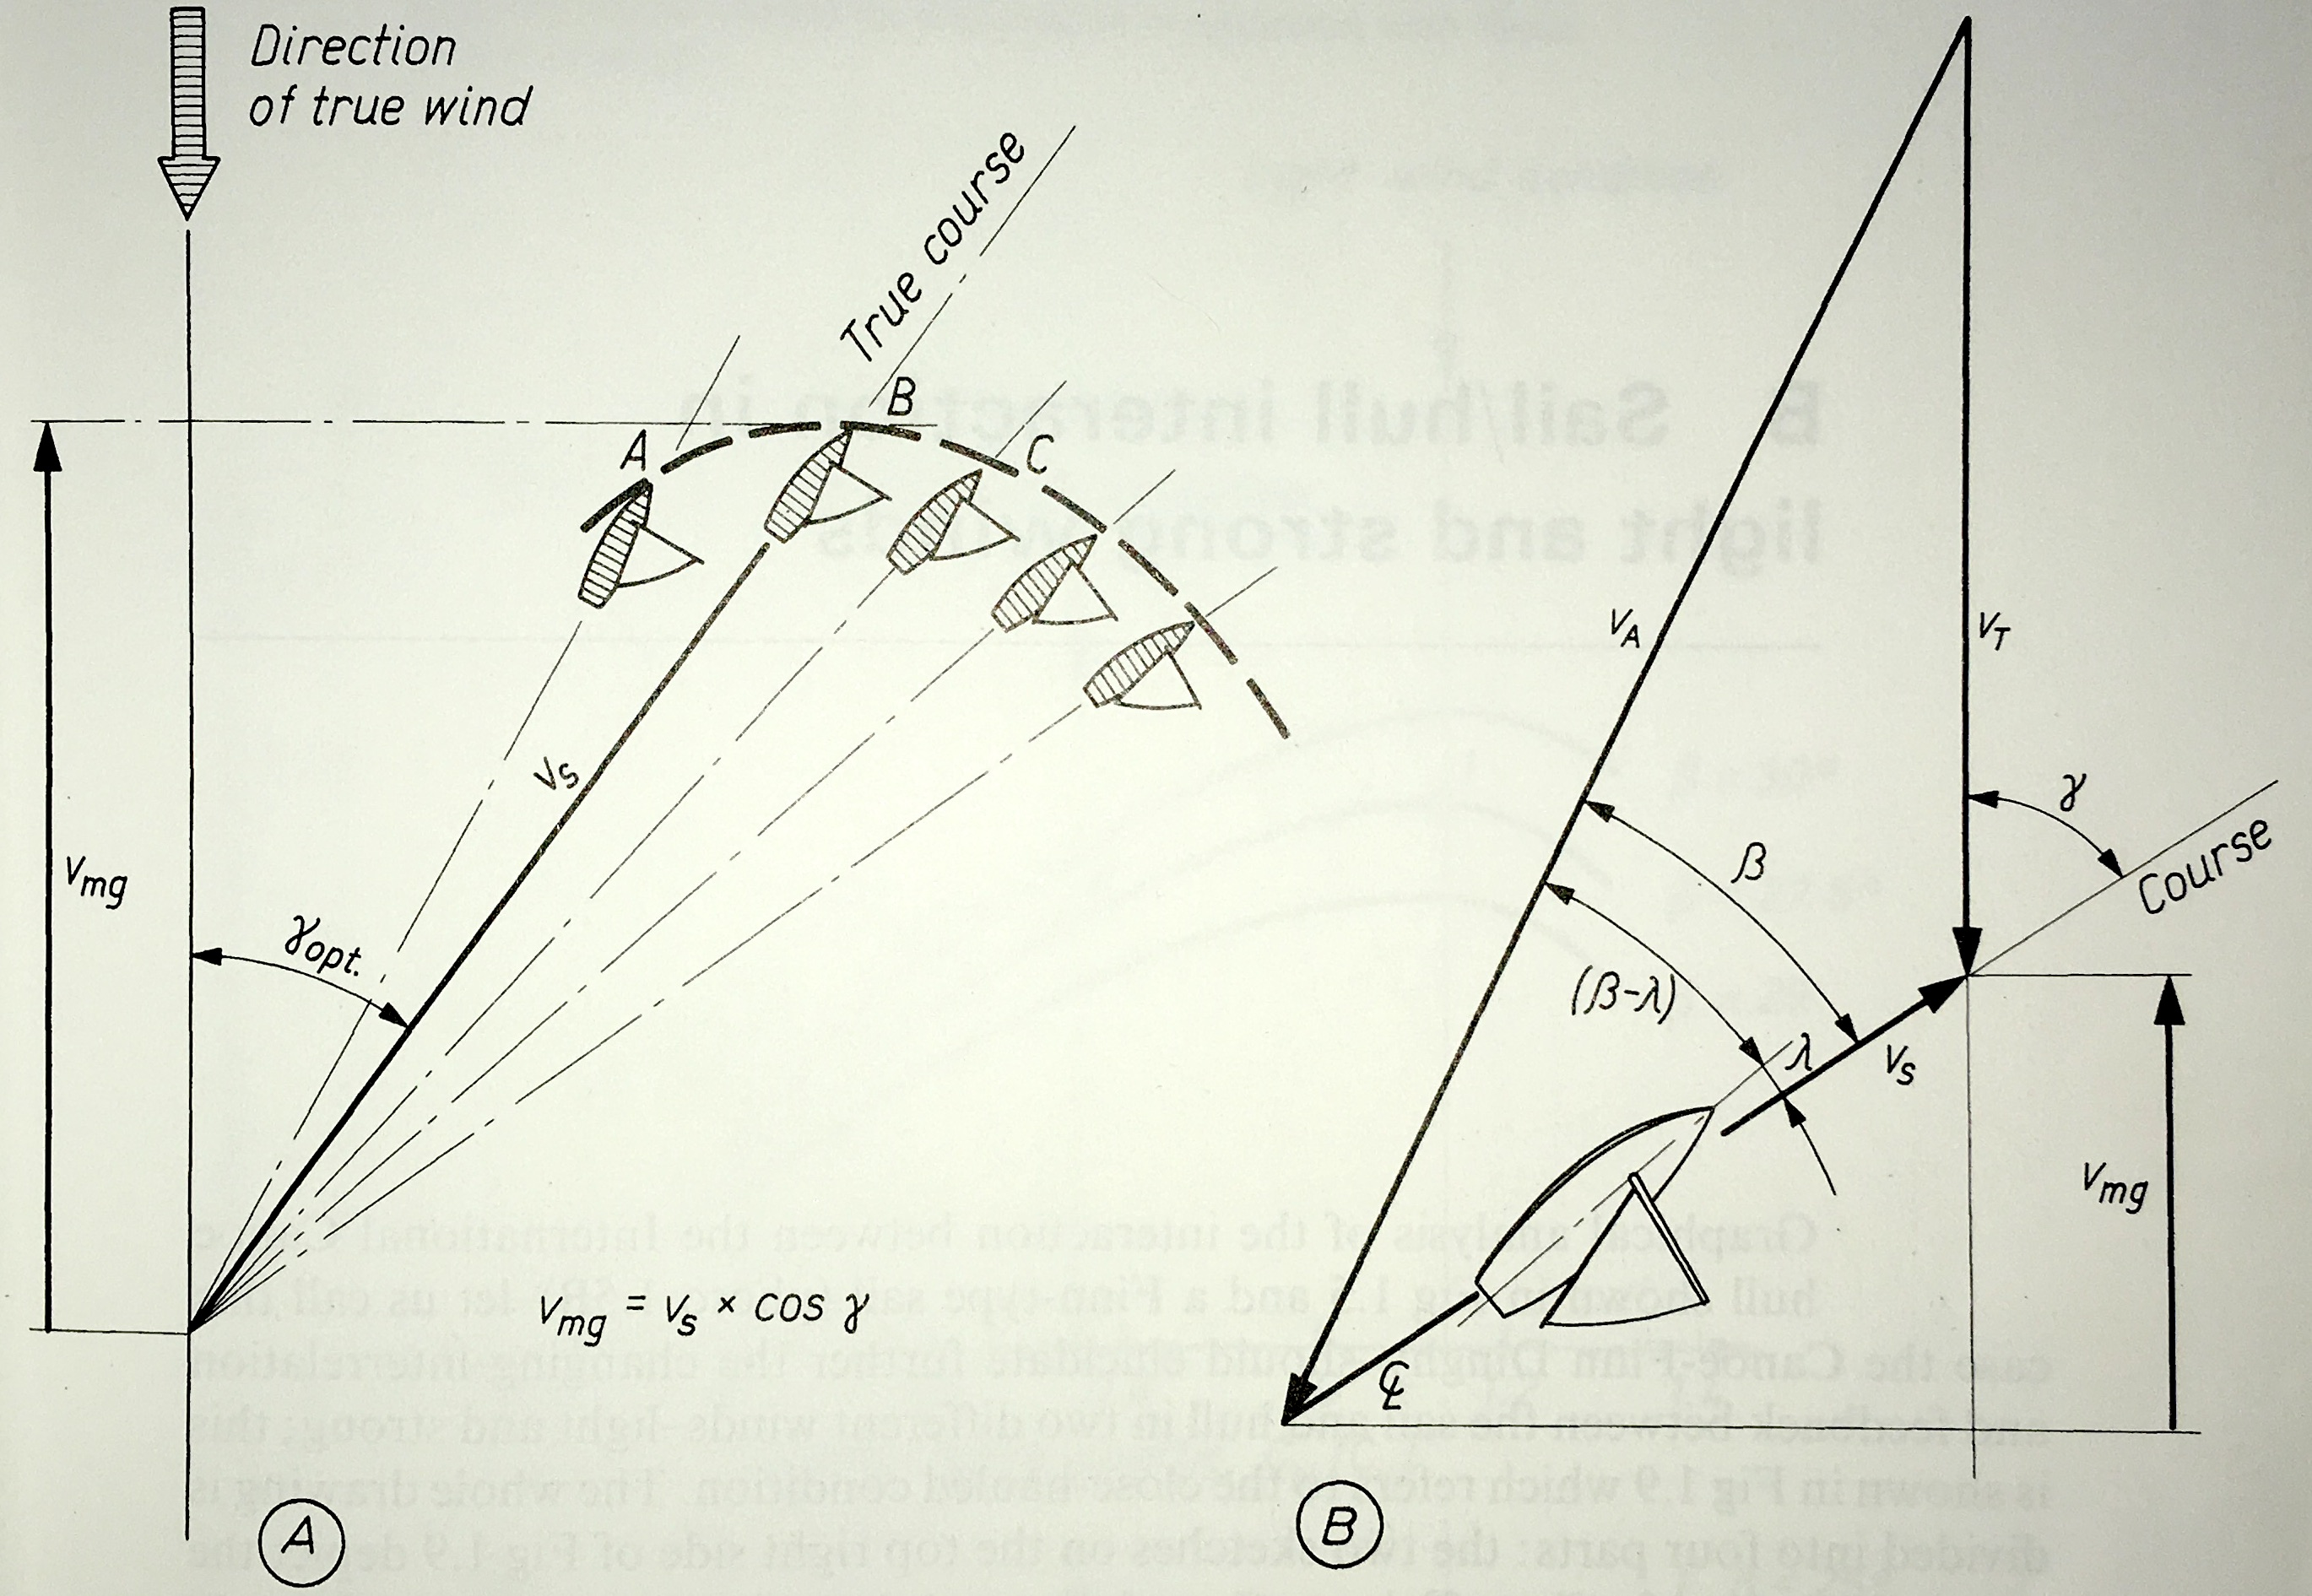
\includegraphics[width=0.75\linewidth]{images/vmg_march.jpeg}
    \caption{Definition of VMG. A. VMG at  different angles. B. Velocity triangle including the leeway angle \cite{marchajaereo1979}.}
    \label{fig:vmg_marchal_book}
\end{figure}
The VPP is obtained by balancing the equations from previous sections, from equation \ref{eq:force_x} to equation \ref{eq:sail_moment}. It derive the $V_{boat}$ at different wind conditions and at different directions, angles respect to the wind. 
%and under  forces and momentum find the a solution which is the velocity of the sailboat and direction respect to the wind, intensity and direction. 
However these equations are not usually solve in its six DOF. Because it was assumed that the vertical forces and moments are always in equilibrium, as was mentioned by \cite{larsonprinciples}, \cite{fossati2009aero} and on section \ref{sec:interaction_boat_environ},  the VPP partially solve the equations which means that the result provided only applies on 2D; particularly in the plane \textit{XY}, so it only considers 2 DOF  because changes on the \textit{Z} plane are neglected; but the variables that affected are considered. In this section, it was identify how the variables are categorized most important which variables can be adjusted by the seamanship and which are defined by the sailboat and weather. 
%the In section was mentiones that it is assumed that the vertical forces and moments are always in equilibriums. 
%Due to this assumption the VPP only solve the equation is a 2D or over the plane XY because changes on the Z plane as neglected. 

\section{Equations of Motion}
The motion of the boat from one point to another occurs in the XY plane. In the previous sections the different components like forces generated by the wind and water were explained and how the seamanship or athlete compensate these forces by interacting with sailboat via sail,$\beta_(tw)$, and rudder, $\lambda$, mainly,. On section \ref{section:forces_moment} %is was explained the interaction of the forces to attained the equilibrium also 
it was mentioned that the  pitching moment and sway forces (vertical forces) are always in equilibrium, which means that heave translation and pitching moment can be omitted and the motion analysis only occurs on the XY plane. \par 

The Eulerian equations of motion for sailboats are taken from \cite{de2004mathematical} and for simplicity the total forces are going to be indicated by the axis direction, and the sub index will indicate the element of the sailboat where it is applied.\newline
\newline
The forces on the X and Y axis are: 
\begin{equation}\label{eq:force_X_motion}
    X_{U}+X_{hull}+X_{rudder}+X_{sail}=m(\Dot{u}-v\Dot{\psi})
\end{equation}
\begin{equation}\label{eq:force_Y_motion}
    Y_{hull}+X_{rudder}+X_{sail}=m(\Dot{v}-u\Dot{\psi})
\end{equation}
And the momentum on the X and Y axis are:
\begin{equation}\label{eq:moment_X_motion}
    K_{hull}+K_{rudder}+K_{sail}+K_{stability}=I_{xx} \Ddot{\phi}
\end{equation}
\begin{equation}\label{eq:moment_Y_motion}
    N_{hull}+K_{rudder}+K_{sail}=I_{zz} \Ddot{\psi}
\end{equation}
%<vertical forces are in balance always same as the pitching moment
where: 
\begin{itemize}  \label{symbols o motions}
 \setlength \itemsep{0em}
\item m = the total mass of the sailboat including crew.
\item u = velocity along the X axis.
\item v= velocity along the Y axis.
\item $\phi$ = roll angle.
\item $\psi$ = yaw angle.
\item $I_{xx}$ = total mass moment of inertia in roll axis (x).
\item $I_{zz}$ = total mass moment of inertia in yaw axis (z).
\item K = Rolling moment (x axis).
\item N = Yawing moment (z axis).
\item $X_{U}$ = is the hull resistance in the upright position.
\item $X/Y_{hull}$ = is the resistance under the heeled hull resistance.
\end{itemize}

The rudder and the sail are the sailboat elements that are controlled by the seamanship. The hull and sail forces are going to explain in detail later in this section. The previous equation were modified by Masuyama to include the hydrodynamics derivatives of the hull \cite{masuyama2011tacking}, with this \cite{de2004mathematical} the mathematical model of the tacking maneuvers represent more accurately the relation and effects of the hydrodynamics forces.\newline
\\
Surge  (x axis):
\begin{multline}\label{eq:force_xMasuyama}
    X_{U}+X_{hull}+X_{rudder}+X_{sail}+X_{V\Dot{\psi}}V\Dot{\psi}\\ =(m+m_{x})\Dot{u}-(m+m_{y}cos^2\phi+m_{z}sin^2\phi)v\Dot{\psi}
\end{multline}
\\
Sway  (y axis):
\begin{multline}
\label{eq:force_yMasuyama}
Y_{hull} + Y_{rudder} + Y_{sail} + Y_{\Dot{\phi}} \Dot{\phi} + Y_{\Dot{\psi}} \Dot{\psi} \\ 
=(m + m_{y})cos^2 \phi + m_{z} sin^2 \phi \Dot{v} + (m + m_{x})u \Dot{\psi} + 2(m_{z} - m_{y}) sin\phi cos\phi \cdot v \Dot{\phi}
\end{multline}
\\
Roll (x axis):
\begin{multline}
     K_{hull} + K_{rudder} + K_{sail} + K_{stability} +K_{\Dot{\phi}} \Dot{\phi} \\
 =(I_{xx} + J_{xx}) \Ddot{\phi} - {(I_{yy} + J_{yy})-(I_{zz} + J_{zz})} sin\phi cos\phi \cdot \Dot{\psi}^2
\end{multline}  \label{eq:m_xMasuyama}
\newline
Yaw (x axis):
\begin{multline}
   N_{hull}+N_{rudder}+N_{sail}+N_{\Dot{\psi}}\Dot{\psi}\\
 ={(I_{yy} + J_{yy}sin^2 \phi +(I_{zz} + J_{zz}cos^2 \phi}\Ddot{\psi} +2{(I_{yy} + J_{yy})-(I_{zz} + J_{zz})}sin\phi cos\phi \cdot \Dot{\psi} \Dot{\phi}  
\end{multline}\label{eq:m_yMasuyama}
\newline
where: 
\begin{itemize}  \label{symbols_motions2}
 \setlength \itemsep{0em}
\item $m_{x/y/z}$ = the added masses in x,y and z direction.
\item $I_{xx}$,$I_{yy}$,$I_{zz}$ = total mass moment of inertia.
\item $J_{xx}$,$J_{yy}$,$J_{zz}$ = total added mass moments of inertia.
\item $X_{V\Dot{\psi}}$, $Y_{\Dot{\psi}}$, $N_{\Dot{\psi}}$  = hydrodynamic derivatives of the hill due to yawing.
\item $Y_{\Dot{\phi}}$, $K_{\Dot{\phi}}$  = hydrodynamic derivatives of the hill due to rolling.
\end{itemize}
